\section{Designing \name}\label{s:design}
%
\cut{
\an{maybe move to ``bundler's utility regime''/Overview/``Traffic Bundles'': 
What is the best way to take advantage of the existence of traffic bundles?
Broadly, there are two approaches: congestion control and in-network scheduling. 
Today, congestion control is a distributed concern: each end-host performs its own optimization to achieve the highest throughput and lowest latency.
Indeed, end-host rate control is a deployed method to enforce domain-wide scheduling policy in private WANs~\cite{bwe}.
On the other hand, scheduling is an in-network concern; existing proposals such as DiffServ~\cite{diffserv} observe that the network is uniquely positioned to differentiate between different flows according to some domain-wide policy.
Scheduling presents its own challenge: because the Internet is a federated system, the link with queue build-up (and thus with the opportunity to re-order packets according to a scheduling policy) will likely be outside the sending domain's purview.

\an{don't know what to say next}
}
}

Recall that in order to do scheduling, we need to move the queues from the network to the \name. 
In this section, we first describe our key insight for moving the in-network queues, and then explain our specific design choices. 
Recall that each site deploys one \name middlebox which we logically partition into sender-side (\inbox) and receiver-side (\outbox) functionality.

\subsection{Key Insight}\label{s:design:key}
We induce queuing at the \inbox by rate limiting the outgoing traffic. 
If this rate limit is made smaller than the bundle's fair share of bandwidth at the bottleneck link in the network, it will decrease throughput. 
Conversely, if the rate is too high, packets will pass through the \inbox without queueing.
Instead, the rate needs to be set such that the bottleneck link sees a small queue while remaining fully utilized (and the bundled traffic competes fairly in the presence of cross traffic). 
We make a simple, but powerful, observation: existing congestion control algorithms calculate exactly this rate~\cite{Jacobson88}. 
Therefore, running such an algorithm to set a bundle's rate would reduce its self-inflicted queue at the bottleneck, causing packets to queue at the \inbox instead, without reducing the bundle's throughput.
Note that end hosts would continue running a traditional congestion control algorithm as before (\eg Cubic~\cite{cubic}, BBR~\cite{bbr}) which is unaware of \name.
Rather, the \inbox's congestion control algorithm acts on the traffic bundle as a \emph{single unit}.

Figure~\ref{fig:design:shift-bottleneck} illustrates this concept for a single flow traversing a bottleneck link in the 
network.\footnote{Details of the emulated network setup which resulted in the illustrated queue length time-series are in \S\ref{s:eval}.}
Without \name, packets from the end hosts are queued in the network, while the queue at the edge is unoccupied. 
In contrast, a \name deployed at the edge is able to shift the queue to its \inbox.

\subsection{System Overview}\label{s:design:overview}
\begin{figure}
    \centering
    \includegraphics[width=\columnwidth]{img/arch-block-diag}
    \vspace{-40pt}
    \caption{\name comprises of six sub-systems: four (in green) implement \inbox functionality, one (in blue) implements \outbox functionality, and the datapath (orange) is shared between the two. \cut{\radhika{should we put the \name blocks inside another box called ``control plane''?}}}\label{fig:design:block-diag}
\end{figure}
%\fc{starts a bit abruptly, better lead in?}
% in order to run congestion control for an aggregation of flows, you need some way to measure the network. 
Figure~\ref{fig:design:block-diag} shows \name's sub-systems: 
(1) A congestion control module at the \inbox which implements the rate control logic and cross-traffic detection, as discussed in \S\ref{s:design:whichcc}.
(2) A mechanism for sending congestion feedback (ACKs) in the \outbox, and (3) a measurement module in the \inbox that computes congestion signals (RTT and receive rate) from the received feedback. We discuss options for implementing congestion feedback mechanism in \S\ref{s:design:twosided} and how to use that feedback in the measurement module in \S\ref{s:measurement}.
(4) A datapath for packet processing (which includes rate enforcement and packet scheduling). Any modern middlebox datapath, \eg BESS~\cite{bess}, P4~\cite{p4}, or  Linux qdiscs (as used in our prototype implementation---see \S\ref{s:impl}), is suitable. 
%\fc{should we add ecmp detection?} \radhika{can we think of it as part of measurement? let's not bring too much attention to it}
We detail the interaction between these subsystems when discussing our prototype implementation in \S\ref{s:impl}. 
%
%\an{radhika, pls check this subsection and the figure. I think it no longer requires understanding how everything works and is more of an overview?}
%\radhika{i think it looks good now! i edited it slightly -- adding more detailed sentences so that it gives a slightly more holistic overview. please check. Also, do you want to update fig 5 to make it even more consistent with this? e.g. in Fig 5, replace `Send Box' with `Measurement', `Receive box' with `Congestion ACKs', `CCP' with `Congestion Control (CCP)'? You can have the terms SendBox and ReceiveBox outside the boxes.}
%Figure~\ref{fig:design:block-diag} shows the necessary components of \name: (1) a means of determining bundle membership; (2) a rate enforcement mechanism; (3) a measurement strategy; (4) a delay-controller; and (5) a fairness-controller.
%Throughout this section we discuss design options for determining Bundle membership (\S\ref{s:design:membership}), observing feedback (\S\ref{s:design:twosided}), and congestion control (\S\ref{s:design:whichcc}): for other aspects of the design, \name is compatible with a variety of options. For example, domains can implement \name using any modern middlebox datapath, \eg P4~\cite{p4}, BESS~\cite{bess}, or as in our prototype implementation (\S\ref{s:impl}), Linux tc qdiscs.
%\radhika{maybe we can chop this subsection off -- let's discuss.}
%
In the rest of this section, we discuss our key design choices.
%Our overarching design principle is simplicity; at various points in the design, there exists a more complex approach which we discard.\fc{why? maybe just remove this?} \radhika{yes, can remove}

\cut{
\subsection{Identifying Bundle Membership}\label{s:design:membership}
\an{I think we can cut this with the site-to-site framing.}
\name must first identify which packets (or flows) are part of the same traffic bundle.
To compute and enforce correct sending rates for a traffic bundle, it is important to only bundle those flows that share the same bottleneck.
%; otherwise, \name may send a component flow at the wrong rate for its bottleneck.
This has traditionally been a difficult problem; 
Rubenstein \etal~\cite{active-sharedbottlenecks} use a ``poisson-probing'' mechanism to probabilistically identify shared bottlenecks under a limited network model, and
multipath TCP~\cite{mptcp} sidesteps it with a weighted window increase-decrease protocol.

Deploying \name boxes close to both endpoints allows us to adopt a more direct (and accurate) approach based on a \emph{two-way opt-in}.
In this approach, a site must agree to bundle traffic on both the sending and receiving sides.
The first step, of course, is to place a \name middlebox at the domain's edge.
Initially, the \inbox assumes all component traffic is unbundled.
When the \outbox observes an unbundled packet, it opts-in by sending an initialization message
\footnote{To avoid sending an initialization message for every unbundled packet, the \outbox samples the unbundled packets using the same mechanism as in \S\ref{s:measurement}.} 
(analogous to TCP's SYN) 
containing the IP prefixes it covers, addressed to the source IP of the packet
\footnote{Addressing to the source IP of the packet is not strictly necessary; domains may also advertise \inbox{}es via \eg DNS.}.
If there is no \inbox on the path, this message will be ignored.
Otherwise, a \inbox will observe this message and can opt-in by initializing a new traffic bundle corresponding to the \outbox's destination prefixes and sending a message (analogous to TCP's SYNACK) notifying the \outbox of the source IP prefixes it covers, so the \outbox can initialize a bundle corresponding to that sending domain.
Now, the \inbox and \outbox can identify packets belonging to initialized bundles by matching the corresponding IP prefixes.
Any subsequent packets the \outbox observes from that sending domain are treated as part of the bundle.

%The \outbox does one of two things for each potential epoch boundary packet:
%\begin{enumerate}
%    \item If the packet is in a known bundle, the \outbox sends a message to the corresponding \inbox.
%    \item If the packet is not in a known bundle, the \outbox sends a message to the source IP address of that packet.
%\end{enumerate}

%The \inbox receives (and intercepts) the \outbox feedback.  
%The \inbox at this time updates its flow tables to add the destination IP of the epoch boundary packet either to an existing bundle (in the case of a new flow from a previously-unseen source subnet joining a bundle) or instantiates a new bundle.
%The \inbox then sends a response containing an epoch size to use and the hash of the epoch boundary packet.
%The \outbox receives this message, initializes a byte counter for the newly discovered bundle, and remembers the \inbox IP address for future feedback. If there is no \inbox on the path, the packet will simply be ignored at its destination. 
}

\subsection{Choice of congestion control algorithm}\label{s:design:whichcc}
\name's congestion control algorithm must satisfy the following requirements: 

\paragraphi{(1) Ability to limit network queueing} \name must limit queueing in the network to move the queues to the \inbox. Therefore, congestion control algorithms which are designed to control delays, and thus queueing, are the appropriate choice. 
A loss-based congestion control algorithm which fills buffers (\eg Cubic, NewReno), for example, is not a good choice for \name, since it would build up a queue at the network bottleneck and drain queues at the \inbox.

\paragraphi{(2) Detection of buffer-filling cross-traffic} It is well known that delay-controlling schemes (\eg Vegas~\cite{vegas}) compete poorly with buffer-filling loss-based schemes~\cite{copa}.
Therefore, \name must have a mechanism to detect the presence of such competing buffer-filling flows and fall back to status quo performance, and then detect when they have left to take back its control over the network queues. 

The emergence of such detection mechanisms is recent: Copa~\cite{copa} detects whether it is able to empty the queues, and Nimbus~\cite{nimbus-arxiv} provides a more general mechanism which overlays a pattern on the sending rate and measures the cross traffic's response.
Copa is not designed for aggregate congestion control (see \S\ref{s:queue-ctl}); thus, we use the more general Nimbus mechanism.

\subsection{Congestion Feedback Mechanism}\label{s:design:twosided}
A congestion control algorithm at the \inbox would require network feedback from the receivers to measure congestion and adjust the sending rates accordingly. We discuss multiple options for obtaining this. 

%This problem presents multiple possible solutions:

\paragrapha{Passively observe in-band TCP acknowledgements}
Conventional endhost-based implementations have used TCP acknowledgements to gather congestion control measurements. A simple strategy for \name is to passively observe the receiver generated TCP acknowledgements at the \inbox. However, we discard this option as it is specific to TCP and thus incompatible with alternate protocols, \ie UDP for video streaming or QUIC's encrypted transport header~\cite{quic}.

\paragrapha{Terminate connections and proxy through TCP} With this approach, one would terminate end-host TCP connections at the \inbox and open new connections to the \outbox, allowing the \inbox to control the rate of traffic in these connections.
%This approach allows the unmodified use of existing congestion control algorithms for the TCP connection between the \inbox and the \outbox \radhika{edited, pls check}. 
%since a TCP tunnel can collect ACKs. 
This approach can improve performance by allowing end-to-end connections to ramp up their sending rates quickly. 
%\radhika{unclear} \radhika{also, wouldn't this approach have the same disadvantage as previous one?}
The primary disadvantage of this approach is that \name must take responsibility for reliable delivery of component traffic, which requires large amounts of queueing and, in the case of UDP applications, can harm application performance. 
Furthermore, proxying TCP connections introduces a new potential point of failure at \name that violates fate-sharing; if \name crashes, connections will be lost.
Finally, from a practical standpoint, to avoid head-of-line blocking this approach requires that \name open a new proxy connection for each component end-host connection, but still determine the bottleneck rate of the traffic \emph{aggregate}. While this approach may be technically feasible~\cite{cm}, it would result in high overhead.
\cut{\footnote{From an architectural standpoint this design runs counter to the end-to-end principle~\cite{e2e-principle}; it replicates endhost functionality in the network.}}
%the cycles used for opening and managing new proxy connections are better used for packet processing.
Thus, we set aside TCP proxies for the remainder of this discussion, but explore their compatibility with \name in \S\ref{s:eval:proxy}. 
%We but note that this approach is complementary with \name (see \S\ref{s:eval}).

%\an{discuss non-terminating tcp tunnels?}
\paragrapha{Out-of-band feedback} Having eliminated the options for using in-band feedback, we adopt an out-of-band feedback mechanism: the \outbox sends out-of-band congestion ACKs to the \inbox.
This decouples congestion signalling from traditional ACKs used for reliability\footnote{The idea of an out-of-band congestion notification is similar to that in QCN~\cite{qcn}, although our goals differ.} and is thus indifferent to the underlying protocol (be it TCP, UDP, or QUIC).
%We detail the congestion measurement strategy and contents of congestion ACKs in \S\ref{s:measurement}.

\cut{
\begin{Appendix}
\section{Nimbus}\label{s:app:nimbus}
\begin{figure*}[ht!]
    \centering
\begin{knitrout}
\definecolor{shadecolor}{rgb}{0.969, 0.969, 0.969}\color{fgcolor}
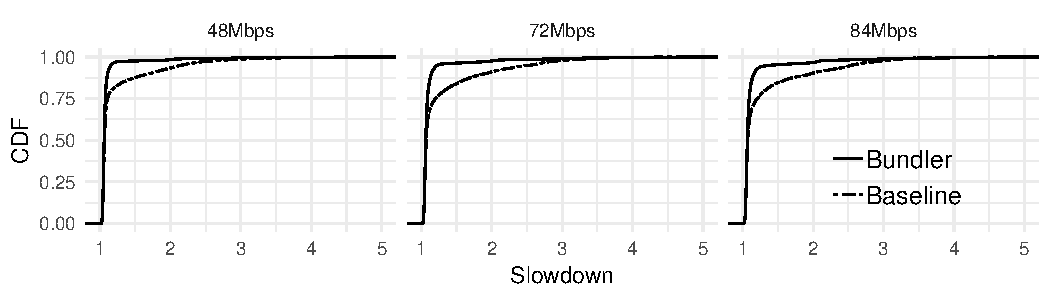
\includegraphics[width=\maxwidth]{figure/eval:offeredload-1} 

\end{knitrout}
    \caption{\name offers diminishing returns with lower amounts of offered load.}
    \label{fig:eval:offeredload}
\end{figure*}
%
%\newcommand{\highUtilTailImprove}{round(highUtilTailImprove, 0)\%\xspace}
%\newcommand{\medUtilTailImprove}{round(medUtilTailImprove, 0)\%\xspace}
%\newcommand{\lowUtilTailImprove}{round(lowUtilTailImprove, 0)\%\xspace}


We briefly summarize Nimbus~\cite{nimbus} for reference.

Nimbus's goal is to detect scenarios in which it is safe to use delay-based congestion control. 
To achieve this goal, Nimbus proposes an \emph{elasticity detector} to detect whether the cross traffic contains any \emph{elastic} flows, which react to changes in the available bandwidth on fast time-scales, \ie a couple RTTs. 
Nimbus's core observation is that the absence of such elastic cross traffic, \ie competition with only \emph{inelastic} traffic, is a sufficient (but not necessary) condition to use a delay-control algorithm.
Nimbus thus measures whether cross traffic reacts to changes in available bandwidth by pulsing its sending rate at a predetermined frequency.
If the cross traffic's rate responds to these pulses at the same frequency, Nimbus can conclude that it is elastic, because it has reacted to changes in the available bandwidth.

A natural method of measuring the cross traffic's frequency response is to compare Nimbus's pulses with the cross traffic's rate in the frequency domain.
Thus, Nimbus uses an asymmetric sinusoidal pulse (as we have noted in \S\ref{s:queue-ctl}) which has a straightforward representation in the frequency domain while maximizing the sender's ability to influence the available bandwidth.

How can Nimbus know the cross traffic's response? It develops an estimator for the cross traffic's sending rate:
\begin{equation}
    \hat{z}(t) = \mu\frac{S(t)}{R(t)} - S(t)
\end{equation}

$\hat{z}(t)i$ is the estimated cross traffic rate, $\mu$ is the estimated bottleneck bandwidth, $S(t)$ is the sending rate, and $R(t)$ is the receiving rate. 
    \name measures $R(t)$ using congestion ACKs from the \outbox and $\mu$ using the maximum receive rate as in BBR~\cite{bbr}.

Then, Nimbus searches for a peak in the neighborhood of its pulsing frequency $f_p$ to determine the elasticity metric $\eta$:

\begin{equation}
    \eta = \frac{|\text{FFT}_{\hat{z}}(f_p)|}{\text{max}_{f \in (f_p, 2f_p)} |\text{FFT}_{\hat{z}}(f)|}
\end{equation}

If $\eta$ is larger, the cross traffic is more elastic.
Nimbus then uses a hard-decision rule $\eta \ge 2$ to decide when to switch to cross-traffic competitive mode as described in \S\ref{s:queue-ctl}.

\end{Appendix}
}

\subsection{Measuring Congestion}\label{s:measurement}
\begin{figure}
    \centering
    \includegraphics[width=\columnwidth]{img/rate-calculation}
    \caption{Example of epoch-based measurement calculation. Time moves from top to bottom.
    %Packets from flows in a bundle
    %pass through the \inbox and \outbox middleboxes on the way to their destination. 
    The \inbox records the packets that are identified as epoch boundaries. 
    The \outbox, up on identifying such packets, sends a feedback message back to
    the \inbox, which allows it to calculate the RTT and epochs.
    %When the \inbox observes a packet header matching the boundary condition, it records it. 
    %When the \outbox observes this packet, it sends an out-of-band feedback message back to
    %the \inbox, which allows it to calculate the RTT and epochs.
    }\label{fig:ratecalc}
\end{figure}

% \name uses out-of-band congestion ACKs to signal congestion between the \inbox and \outbox. 
% %Sending these congestion ACKs up on every packet is not just unnecessary, but also incurs high overhead. The \outbox instead sends congestion ACKs only for a few sampled packets. We refer to the period between two successively sampled packets as an \emph{epoch}, and each sampled packet as an \emph{epoch boundary packet}.
% We answer the following questions: (1) When should the \outbox send congestion ACKs? (2) What information should the congestion ACKs contain?

% \subsection{Timing of Congestion ACKs}
% \label{s:measure:marking}
% \newcommand{\pone}{$p_{i-1}$}
% \newcommand{\hpone}{$h(p_{i-1})$}
% \newcommand{\sone}{$s_{i-1}$}
% \newcommand{\rone}{$r_{i-1}$}
% \newcommand{\ptwo}{$p_{i}$}
% \newcommand{\hptwo}{$h(p_{i})$}
% \newcommand{\stwo}{$s_{i}$}
% \newcommand{\rtwo}{$r_{i}$}
% \newcommand{\atwo}{$a_{i}$}
% \newcommand{\sentone}{$sent_{i-1}$}
% \newcommand{\recvdone}{$rcvd_{i-1}$}
% \newcommand{\senttwo}{$sent_{i}$}
% \newcommand{\recvdtwo}{$rcvd_{i}$}

%\an{I think it would be possible to roll this into 4.5}
Sending an out-of-band feedback message for every packet arriving at the \outbox would result in high communication overhead. 
Furthermore, conducting measurements on every outgoing packet at the \inbox would require maintaining state for each of them, which can be expensive, especially at high bandwidth-delay products. 
This overhead is unnecessary; reacting once per RTT is sufficient for congestion control algorithms~\cite{ccp}. 
The \inbox therefore samples a subset of the packets for which the \outbox sends congestion ACKs.
We refer to the period between two successively sampled packets as an \emph{epoch}, and each sampled packet as an \emph{epoch boundary packet}.

The simplest way to sample an epoch boundary packet would be for the \inbox to probabilistically modify a packet (\ie set a flag bit in the packet header) and the \outbox to match on this flag bit.
However, where in the header should this flag bit be?
Evolving packet headers has proved impractical~\cite{trotsky}, so perhaps we could use an encapsulation mechanism.
Protocols at both L3 (\eg NVGRE~\cite{nvgre}, IP-in-IP~\cite{ipinip}) and L4 (\eg VXLAN~\cite{vxlan}) are broadly available and deployed in commodity routers today.

Happily, we observe that such packet modification is not inherently necessary; since the same packets pass through the \inbox and \outbox, uniquely identifying a given pattern of packets is sufficient to meet our requirements. In this scheme, the \inbox and \outbox both hash a subset of the header for every packet, and consider a packet as an epoch boundary if its hash is a multiple of the desired \emph{sampling period}.
% The \inbox computes the sampling period to produce about 4 samples per RTT and communicates it to the \outbox.
%We defer the details of sampling period computation to Appendix~\ref{app:epochs}. 

Upon identifying a packet $p_i$ as an epoch boundary packet the \inbox records: 
(i) its hash, $h(p_i)$, 
(ii) the time when it is sent out, $t_{\text{sent}}(p_i)$, 
and (iii) the total number of bytes sent thus far including this packet, $b_{sent}(p_i)$. 
When the \outbox sees $p_i$, it also identifies it as an epoch boundary and sends a congestion ACK back to the \inbox. 
The congestion ACK contains $h(p_i)$ and the running count of the total number of bytes received for that bundle. 
Upon receiving the congestion ACK for $p_i$, the \inbox records the received information, and using its previously recorded state, computes the RTT and the rates at which packets are sent and received, as in Figure~\ref{fig:ratecalc}.

\paragrapha{Epoch boundary identification}
The packet header subset that is used for identifying epoch boundaries must have the following properties:
(i) It must be the same at both the \inbox and the \outbox.
(ii) Its values must remain unchanged as a packet traverses the network from the \inbox to the \outbox (so, for example, the TTL field must be excluded).\footnote{Certain fields, that are otherwise unchanged within the network, can be changed by NATs deployed within a site. Ensuring that the \name boxes sit outside the NAT would allow them to make use of those fields.}
(iii) It differentiates individual \emph{packets} (and not just flows), to allow sufficient entropy in the computed hash values.
(iv) It also differentiates a retransmitted packet from the original one, to prevent spurious samples from disrupting the measurements (this precludes, for example, the use of TCP sequence number).
%
We expect that the precise set of fields used will depend on specific deployment considerations.
For example, in our prototype implementation (\S\ref{s:impl}) we use a header subset of the IPv4 IP ID field and destination IP and port. 
We make this choice for simplicity; it does not require tunnelling mechanisms and is thus easily deployable, and if \name fails, connections are unaffected. 
We note that previous proposals~\cite{ip-traceback} have used IP ID for unique packet identification. 
The drawback of this approach is that it cannot be extended to IPv6.
To support a wider set of scenarios, \name could use dedicated fields in an encapsulating header (as in~\cite{axe}).
%\radhika{can we cite something for schemes that have used this before?}

To visualize how these measurements impact the behavior of the signals over time we pick an experiment for which the median difference matches that of the entire distribution and plot a five second segment of our estimates compared to the actual values in Figure~\ref{fig:micro:time-thru}.

\begin{figure}
    \centering
\begin{knitrout}
\definecolor{shadecolor}{rgb}{0.969, 0.969, 0.969}\color{fgcolor}
\includegraphics[width=\maxwidth]{figure/micro:time-thru-1} 

\end{knitrout}

\begin{knitrout}
\definecolor{shadecolor}{rgb}{0.969, 0.969, 0.969}\color{fgcolor}
\includegraphics[width=\maxwidth]{figure/micro:dist-thru-1} 

\end{knitrout}

    \caption{\name's estimate of the receive rate.}
    \label{fig:micro:time-thru}
\end{figure}
 % actually contains the time series

\paragrapha{Choosing the epoch size}
In order to balance reaction speed and overhead, epoch packets should be spaced such that measurements are collected approximately once per RTT~\cite{ccp}.
Therefore, for each bundle, we track the minimum observed RTT ($minRTT$) at the \inbox and set the epoch size $N = (0.25 \times minRTT \times send\_rate)$, where the $send\_rate$ is computed as described above. The measurements passed to the congestion control algorithms at the \inbox are then computed over a sliding window of epochs that corresponds to one RTT. Averaging over a window of multiple epochs also increases resilience to possible re-ordering of packets between the \inbox and the \outbox, which can result in them seeing different number of packets between two epochs.

When the \inbox updates the epoch size $N$ for a bundle, it needs to send an out-of-band message to the \outbox communicating the new value. To keep our measurement technique resilient to potential delay and loss of this message, the epoch size $N$ is always rounded down to the nearest power of two. Doing this ensures that the epoch boundary packets sampled by the \outbox are either a strict superset or a strict subset of those sampled by the \inbox. The \inbox simply ignores the additional feedback messages in former case, and the recorded epoch boundaries for which no feedback has arrived in the latter.  

\paragrapha{Robust to packet loss}
Note that our congestion measurement technique is robust to a boundary packet being lost between the \inbox and the \outbox. In this case, the \inbox would not get feedback for the lost boundary packet, and it would simply compute rates for the next boundary packet over a longer epoch once the next congestion ACK arrives.

\begin{figure}
    \centering
\begin{knitrout}
\definecolor{shadecolor}{rgb}{0.969, 0.969, 0.969}\color{fgcolor}
\includegraphics[width=\maxwidth]{figure/micro_time-delay-1} 

\end{knitrout}

    \caption{\name's estimate of the delay }
    \label{fig:micro:time-delay}
\end{figure}
 % actually contains the distributions
\paragrapha{Microbenchmarks}
To evaluate the accuracy and robustness of this measurement technique, we picked 90 traces from our evaluation covering a range of link delays (20ms, 50ms, 100ms) and bottleneck rates (24Mbps, 48Mbps, 96Mbps), and computed the difference, at each time step, between \name's measurements (estimate) and the corresponding values measured at the bottleneck router (actual). 
In Figure~\ref{fig:micro:time-delay} we focus on the RTT measurements: the bottom plot shows the distribution of the differences, and the top plot puts it into context by showing a five second segment from a trace where the median difference matched that of the full distribution. In Figure~\ref{fig:micro:time-thru}, we produce the same plots for the receive rate estimates.
In summary, 80\% of our RTT estimates were within 1.2ms of the actual value, and 80\% of our receive rate estimates were within 4Mbps of the actual value.


\subsection{Implications of \name's Design}

Our design choices result in an architecture where \name's inner rate control loop can be implemented entirely the ``control plane'' of the \inbox and the \outbox, which passively observes the packets traversing the datapath of the middleboxes, without modifying them. This results in a truly transparent system, that is light-weight, has low overhead, preserves fate-sharing, and in no way interferes with the end-to-end controllers of individual flows. The only datapath action that \name performs is the enforcement of the desired scheduling and queue management policies at the \inbox. 
%\radhika{added this subsection, since i think we weren't emphasizing on this enough. feel free to cut if running out of space.}